\section{Theoretische Grundlagen}
    Eine Maprota besteht aus einer festen Anzahl an Layern mit verschiedenen Gamemodes. 
    Zu beginn der Abfolge wird noch eine feste Anzahl an Seedmaps gelistet welche jedoch für die Mapverteilung des Rota-Generators statistisch irrelevant sind.
    Die folgenden Abschnitte beschäftigen sich mit den benutzten mathematischen Modellen und definiert alle notwendigen Objekte.
    Der genaue Aufbau des Generators ist im nächsten Kapitel zu finden.
    \subsection{Wahrscheinlichkeitsmaß}
        Wie im vorherigen Kapitel dargelegt ist das Ziel eine Mapverteilung zu bekommen welche einer vorgegebenen Verteilung folgt und lokal ein ''Gedächtnis'' besitzt.
        Die vorgegebene Verteilung wird aus den Layervotes generiert, kann aber prinzipiell jede beliebge diskrete Wahrscheinlichkeitsverteilung 
        \begin{equation}
            p_{M,\text{fi}}(m) := \sum_{i=1}^N \mathbb{P}(M=m)
        \end{equation}
        sein, wobei $\mathbb{P}(M=m)$ die Wahrscheinlichkeit ist dass die Map $m$ gezogen wird, repräsentiert durch die Zufallsvariable $X$.
        Das ''Gedächtnis'' wird im folgenden als \textbf{Memory Kernel} bezeichnet.
        Um die obige Verteilung $p_{x,\text{fi}}(x)$ zu realisieren werden mehrere intere Weights verwendet um ein auf System zu repräsentieren welche sich aus mehreren Stufen des ''Ziehens'' eines Gamemodes/Map/Layers zusammensetzt.
        Die Maprota wird dann durch folgende multivariate Verteilung modelliert
        \begin{align}
            p_{G,M,L}(g,m,l)    &= P(G=g, M=m, L=l) \\
                                &= P(G=g)\cdot P(M=m|G=g) \cdot P(L=l|G=g, M=m)
        \end{align}
        wobei $G,M,L$ die Zufallsvariablen \glqq{}Gamemode\grqq{}, \glqq{}Map\grqq{} und \glqq{}Layer\grqq{} sind und $P(A|B)$ die bedingte Wahrscheinlichkeit für das Ereignis $A$ unter der Nebenbedingungen das zuvor $B$ eingetreten ist.
        Die Wahrscheinlichkeit für ein Layer wie \glqq{}Yehorivka RAAS v3\grqq{} ist damit gegeben durch 
        \begin{equation*}
            \mathbb{P}(\text{''Yehorivka RAASv3''}) = p_{G,M,L}(\text{''RAAS'', ''Yehorivka'', ''RAASv3''})
        \end{equation*}
        Das Ziel ist die einzelnen bedingten Wahrscheinlichkeiten so zu wählen, dass wir die Übereinstimmung
        \begin{equation}
            p_{M,\text{fi}}(m) \equiv \sum_{g,l}p_{G,M,L}(g,m,l)
        \end{equation}
        haben, oder zumindest in einer Umgebung dieser Lösung sind definiert durch 
        \begin{equation}
            \sum_m |p_{M,\text{fi}}(m)-\sum_{g,l}p_{G,M,L}(g,m,l)|<\epsilon  
        \end{equation}
        für $\epsilon>0$ aber $\epsilon << 1$.
        \subsubsection{Mode Wahrscheinlichkeiten}
            Die Modewahrscheinlichkeiten definiert durch $p_G(g)=\mathbb{P}(G=g)$ werden \textit{a priori} gesetzt da das Ziehen des Gamemodes der erste Schritt in der Rota-Generierung ist.
            Prinzipiell kann diese von Hand gesetzt werden. 
        \subsubsection{Map Wahrscheinlichkeiten}
            Die Mapwahrscheinlichkeiten              
        \subsubsection{Verteilungsfunktionen}
        Die Gamemode-Wahrscheinlichkeiten werden von Hand gesetzt. 
        Sollte eine Map $m$ nicht im Gamemode $g$ vorhanden sein, so ist die bedingte Wahrscheinlichkeit $P(M=m|G=g) = 0$. 
        Falls die Map vorhanden ist so wird die Wahrscheinlichkeit zum ziehen der Map errechnet aus den Mapvotes verglichen mit den anderen Maps und der Ähnlichkeit zu den zuvor gezogenen Maps.
        Wenn eine Map $m$ gezogen wurde wird ein Layer $l$ nach der Verteilung der Mapvotes der in frage kommenden Layern gezogen. 
        Es ist dann gegeben durch 
        \begin{equation}
            \mathbb{P}(\text{''Layer A''}) = \frac{S(v_i)}{\mathcal{N}}
        \end{equation}
    \subsection{Oberflächliches Model - Baumdiagramm}
        Die statistische Natur der Maprota kann als \glqq{}Würfeln\grqq{} verschiedener Layer verstanden werden. 
        Der Algorithmus setzt sich aus zwei Schichten zusammen: Zunächst wird ein Modus gezogen z.b. \glqq{}Invasion\grqq{}. 
        Die Wahrscheinlichkeit dass ein Modus gezogen wird ist \textit{a priori} gesetzt und wird als externe Größe in den Generator gegeben.
        Nach ziehen des Modus folgt nun die Auswahl der Map. 
        Die Wahrscheinlichkeit das eine Map gezogen wird hängt von den Mapvotes ab und weiteren internen Parametern. 

        \begin{figure}
            \begin{forest}
                for tree={
                  math content,
                  if n=0{coordinate}{circle,draw=black,fill=red!10},
                  grow=0,
                  l=3cm
                }
                [
                 [\overline{A},edge label={node[midway,below=2pt]{$q_1$}}
                  [\overline{D},edge label={node[midway,below]{$p_{21}$}}
                   [\overline{L},edge label={node[midway,below]{$l_{211}$}}]
                   [L,edge label={node[midway,below]{$l_{212}$}}]
                  ]
                  [D,edge label={node[midway,above]{$p_{22}$}}] 
                 ]
                 [A,edge label={node[midway,above=2pt]{$q_2$}}
                  [\overline{D},edge label={node[midway,below]{$p_{11}$}}]
                  [D,edge label={node[midway,above]{$p_{12}$}}] 
                 ]
                ]
            \end{forest}
        \caption{Baumdiagramm zur Zusammensetzung der Mapwahrscheinlichkeiten. 
        Die Wahrscheinlichkeiten, einen Mode zu ziehen, sind $q_1$ und $q_2$ für Mode $1$ und $2$ repsektiv.
        Die Wahrscheinlichkeit, eine Map unter gegebenen Modus zu ziehen, ist gegeben durch $p_{ij}$, d.h. $p_{12}$ ist die bedingte Wahrscheinlichkeit dass Map $2$ gezogen wird wenn vorher Mode $1$ gezogen wurde.}
        \end{figure}
    \subsection{Mapvoteweights}
        Zur Realisierung der Verteilung werden Mapwahrscheinlichkeiten benötigt. 
        Diese werden aus den Layervotes wie folgt gewonnen:\\
        Sei $\mathcal{M}$ die Menge aller Maps. 
        Desweiteren sei $v\in\mathbb{Z}$ die Anzahl an Votes eines Layers.
        Dann wird das Weight für ein $m\in \mathcal{M}$ berechnet nach 
        \begin{align*}
            \mu_i &= \frac{1}{N}\sum_{i=1}^N v_i\\
            w_i &= \exp\left(-(\mu_i-v_i)^2\right)\\
            \bar{w}_i &= \frac{w_i}{\sum_i w_i}\\
            \bar{v}_\text{map} &= \sum_{i=1}^N\bar{w}_i\cdot v_i
        \end{align*}
        Der Mapvote einer Map für einen Modus errechnet sich als das gewichtete arithmetische Mittel aller Votes im selben Modes der Map.
        Das Gewicht eines Votes ist so definiert dass Vote-summen fern des Erwartungswertes weniger stark ins Gewicht fallen.
        Damit soll verhindert werden, dass einzelne \glqq{}Ausreißer\grqq{} die globale Map-Bewertung zu sehr herunterziehen.
        \begin{figure}[htbp]
            \centering
            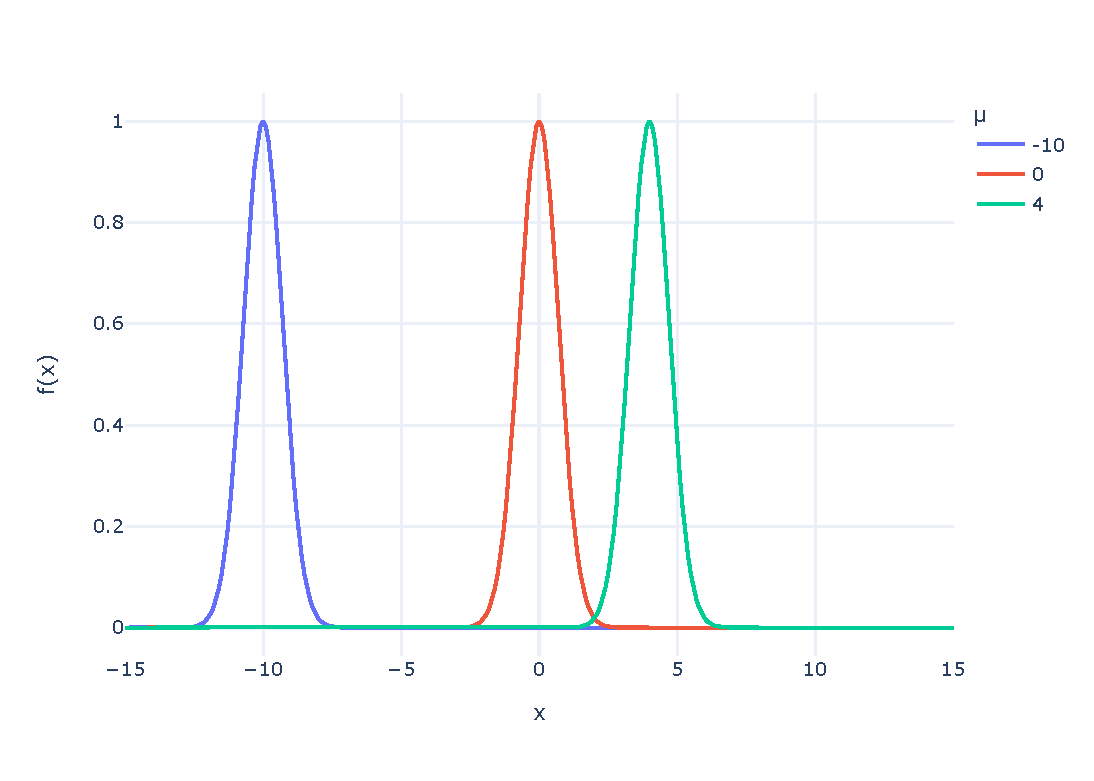
\includegraphics[width=0.85\textwidth]{plot_gaus.pdf}
            \caption{Die Weightfunktion $w_i=f(x)$ geplottet für verschiedene Erwartungswerte.
            Je weiter die Vote-Anzahl vom Mittelwert entfernt ist desto kleiner ist das errechnete Weight und das Layer wird somit stärker bestraft und als ''Ausreißer'' gewertet.}
        \end{figure}
        \subsection{Die Kugel}
    % was muss hier erklärt werden
    % was ist eine rota
    % Überblick aus dem Game, was sind modes was sind map was sind layer, was sind biome 
    % kleine einführung in mathe 
    % was ist eine gute und eine schlechte rota
    Um den ''Map-Charakter'' verschiedener Maps zu vergleichen, werden zunächst verschiedene Charakteristiken definiert wie zum Beispiel ''Wüste'' oder ''Stadt''.
    Jede Map wird ein Anteil an jeder Charakteristik zwischen $0$ und $1$ zugeschrieben, was respektiv dafür steht dass die Eigenschaft gar nicht oder absolut zutrifft für die Map.
    Zum Beispiel würde eine Map mit ''Winter-Setting'' welche nur aus Gebirge besteht in jeder der beiden Eigenschaften den Wert $1$ erhalten. 
    Die Bewertung der einzelnen Maps ist jedoch subjektiv.
    Um den Vergleich zweier Maps zu schaffen wird das System wiefolgt repräsentiert:
    Zu jeder Map $m$ existiert ein ''Biom-Vektor'' $\vec{b} = (b_1,.....,b_n)^T$. 
    Hier stehen die Vektorkomponenten $b_i$ für die obengenannte Zuordnung der entsprechenden Charakteristik und $n$ ist die Anzahl der Vorhandenen Charakteristiken.
    Anschließend wird der Vektor normiert sodas $|\vec{b}|=1$.
    Dadurch wird genau genommen wird der Raum aller Maps-Charakteristiken definiert durch die Hyperfläche
    \begin{equation*}
        \mathcal{L} = \{\vec{x}\in\mathbb{R}^n ||\vec{x}|=1 \land 0\leq x_i \leq \smash{\frac{\pi}{2}} \quad \forall i\in\{1...n\}\}
    \end{equation*}
    Das bedeutet, dass die Maps durch Punkte auf dem Rand der $1/2^n$-tel Kugel beschrieben werden.

    Zwei Maps sind ''ähnlich'', sofern die Punkte nahe beieinander liegen, da in diesem fall die Vektorkomponenten fast alle gleich sind wodurch sich die beiden Vektoren lediglich um einen kleinen Winkel unterscheiden.
    Da die Vektoren normiert sind, entspricht dies einer kleinen Distanz auf der Kugeloberfläche.
    Die Distanz $l$ zweier Punkte auf der Kugel wird im Mapweight verrechnet und ist gegeben durch 
    \begin{equation}
        d = 2\arccos(\vec{a}\cdot\vec{b})
    \end{equation}
    für zwei Map-Charakteristiken $\vec{a}$ und $\vec{b}$, wobei $\cdot$ das innere Produkt (''Skalar Produkt'') bezeichnet. 
    \subsection{Mapweight}
    Das Weight errechnet sich als Produkt aus einem ''Distanz-Weight'' und einem ''Mapvote-Weight''. 
    \begin{equation}
        w_m(m,d,v) = \frac{1}{\mathcal{N}}w_d(d,m)w_v(v,m)
    \end{equation}
    wobei $\mathcal{N}$ das Produkt-Weight normiert sodass $\sum_m w_m = 1$.
    \subsubsection{Distanzweight}
        Das Distanzweight ist eine allgemeine stückweise stetige Funktion definiert durch
        \begin{equation}
            w_d : \mathbb{R}^+ \rightarrow \mathbb{R}^+, d \mapsto w_d(d),
        \end{equation}
        und der Nebenbedingung $w_d(d)\overset{d\rightarrow 0}{\longrightarrow}0$.
        In der momentanen Version ist die Funktion gegeben durch
        \begin{equation}
            w_d(d) = 1_{[0,d_\text{min}]}(d)
        \end{equation}
        mit $d_\text{min}\geq 0$ als Mindestdistanz. 
        Sollte eine Map näher als $d_\text{min}$ an einer zuvor gezogenen Map liegen ist das Distanzweight und damit das Mapweight $0$ und wird damit nicht gezogen. 
    \subsubsection{Mapvoteweight}
        Das Mapvoteweight wird aus dem Mapvote berechnet unter Nutzung einer Sigmoid funktion. 
        \begin{equation}
            w_v(v) = \frac{1}{1+\exp\left(-(av+b)\right)}
        \end{equation}
        wobei $v$ die Summe aller Layervotes eines Modus einer Maps ist und $a$ und $b$ zwei freie Parameter sind.
        Während $a$ die Steigung moduliert kann mit $b$ ein Offset erzeugt werden.
        Die Sigmoid funktion erlaubt es ein kontinuierliches weight zu definieren wodurch eine Map oder ein Layer nicht abrupt verschwindet sondern langsam ändert.
        \begin{figure}[htbp]
            \centering
            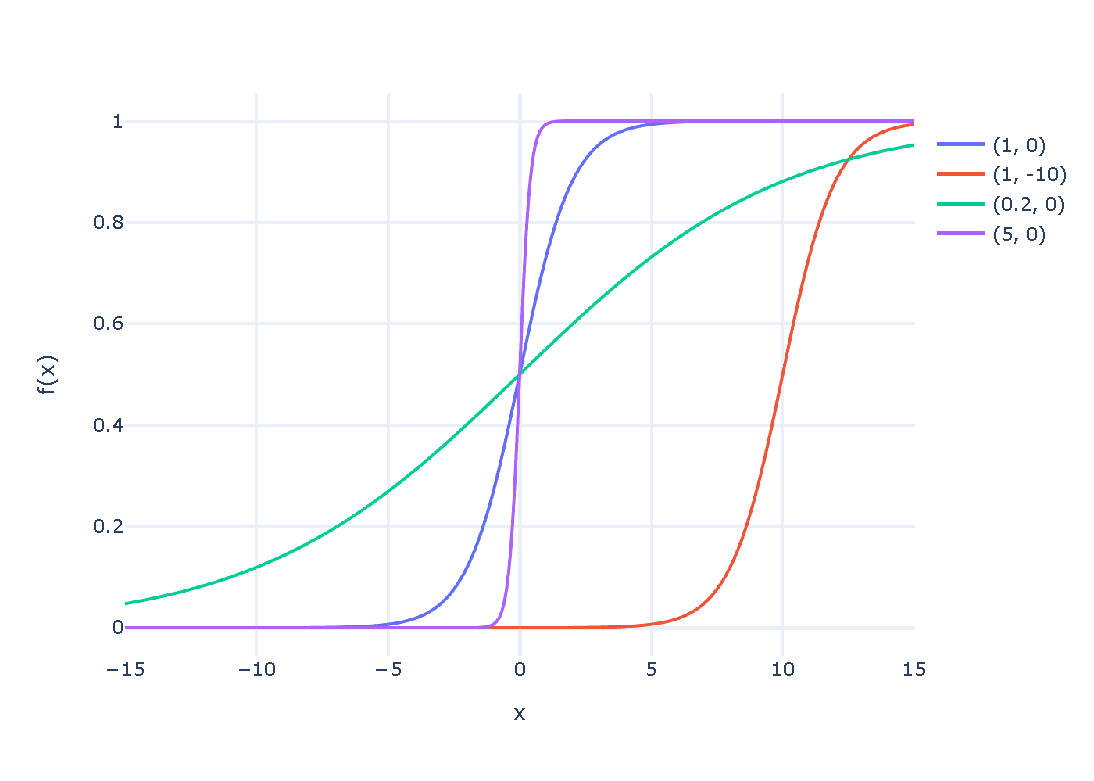
\includegraphics[width=0.85\textwidth]{plot_sigmoid.pdf}
            \caption{Die Sigmoidfunktion für mehrere Werte $a$ und $b$. 
                        Für $b=0$ ist für alle Werte $a$ $f(0)=1/2$.
                        Der Parameter $b$ dient als Offset.}
        \end{figure}
        \todo{sigmod abbildung nicht in text eingebunden}
    \subsection{Zusammenfassung}

    % was ist eine kugel und was meint tim damit 
    % wie werden die mapvotes ausgerechnet
